%%
\chapter{MeerKAT L-Band Primary Beams: Effects of HI Intensity Mapping} \label{Chapter5} 
%% Main chapter title

 % For referencing the chapter elsewhere, use \ref{Chapter1} 

\textbf{Overview}\\
% \HRule \\[0.4cm]
\par\noindent\rule{\textwidth}{0.4pt}\\
\textit{This chapter introduces us to the Zernike model and how it can be used to reconstruct a realistic beam model using
the strongest coefficients (selected number of Zernike coefficients) with corresponding basis patterns. An intensity mapping experiment is performed with these
primary beams to evaluate the angular power spectrum of 21 cm signal.
}%\\
% \HRule \\[1.5cm]
\par\noindent\rule{\textwidth}{0.4pt}
%%

\noindent \texttt{Author’s comment:} 
\small{The primary beam model used in this chapter is part of the work in: K. M. B. Asad, J. N. Girard, M. de Villiers, \textbf{T. Ansah-Narh}, K. Iheanetu, O. Smirnov, M. G. Santos, and others, Primary Beam Effects of Radio Astronomy Antennas – II. Modelling the MeerKAT L-band Beam using Holography. The Monthly Notices of the Royal Astronomical Society (MNRAS), accepted. We therefore confirm that part of the wording in this chapter will  “match” that of the paper. Hence, this note serves as a universal reference for all such text.}

%%
\section{Introduction}	   \label{chap5:intro}
%%

The completely operational MeerKAT instrument is situated in Karoo (a desert area) of South Africa and, is  made up of $64$ \enquote*{offset Gregorian} interferometer. The measurement across the main dish is $13.5 \, \rm m$, that of the secondary reflector is $3.8 \, \rm m$  and, has a maximum separation of $8\, \rm km$.
Almost $70\%$ of the receptors are found in the core area of $1 \, \rm km$ in width. The central location of the interferometer is at latitude $-30\rm d42\rm m47.41\rm s$ and longitude $21\rm d26\rm m38.00\rm s$. There are four feeds on each receptor with the L-band having a frequency range of $0.9 - 1.67\, \rm GHz$.
It also has digitisers supported on the feed indexer. The offset design of MeerKAT provides a better aperture efficiency, a symmetric beam pattern with a decrease in the side-lobes and an increase in the antenna gain. 
The relatively small diameter of the MeerKAT antennas coupled with the large number of antennas and large total collecting makes it a powerful wide-field imaging instrument, with a combination of large field-of-view, wide-bandwidth, high sensitivity and outstanding sampling of the Fourier transform of the sky with 2016 instantaneous baseline samples.

Fig.~\ref{fig:meerkat_layout} displays the station layout of the MeerKAT elements with the left panel showing the representation of the outermost layout and  that of the right panel showing the innermost layout. 
\noindent Refer to \citep{jonas2018meerkat,2018PhyW...31h...8M,2018SPIE10704E..1UR,Santos:2017qgq,taylor2017mightee} for further reading on the design of MeerKAT and its capabilities for science research.

%
%	+++++++++++++++++++++++++++++++++++++++++++
%	MeerKAT Layout
%	++++++++++++++++++++++++++++++++++++++++++++
%
\begin{figure}[ht]
    \centering	    
    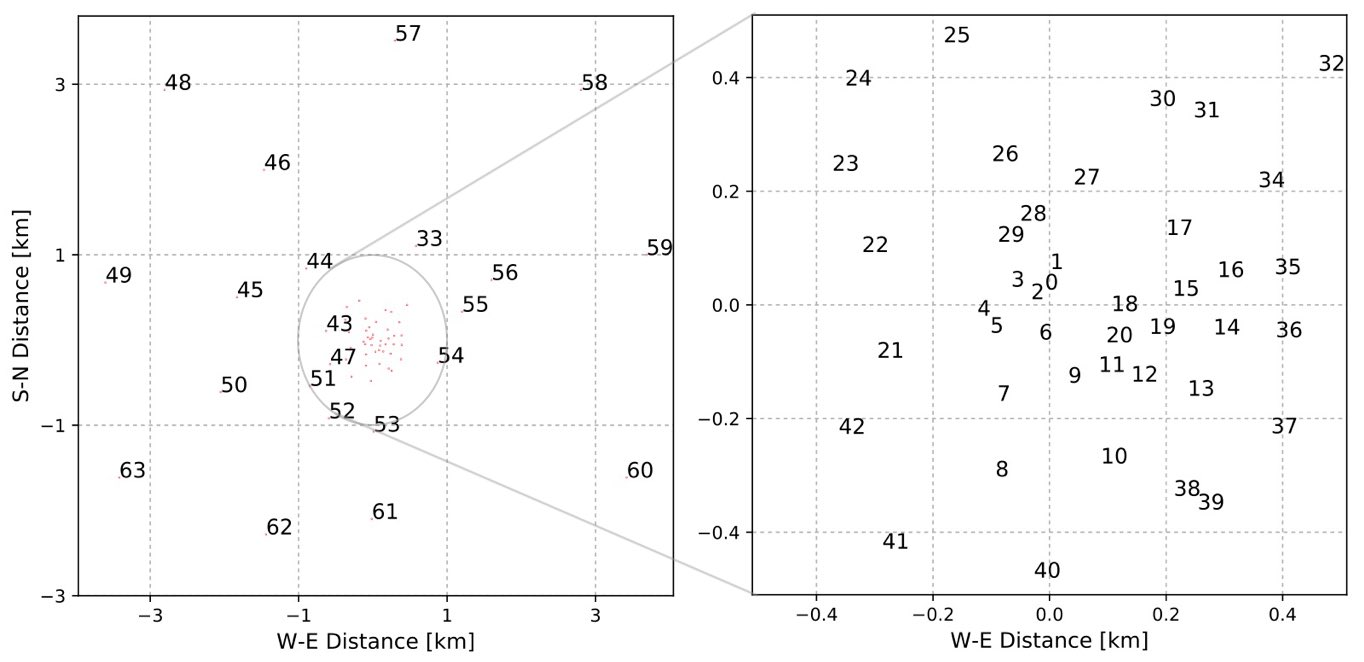
\includegraphics[width=5.8in]{c5/meerkat_layoutt}	    	   
    \caption{The distribution of the 64 antennas of MeerKAT, each identified by an integer ranging from 0 to 63. Note that the actual names of the antennas are given as M000, M001, M002 and so on. Left: The distribution outside the 1 km core. Right: The distribution inside the 1 km  core is loosely delimited by a hexagonal boundary. The West-East and South-North distances are shown relative to the arbitrary centre located at −30d42m47.41s South, 21d26m38.00s East.}
	    \label{fig:meerkat_layout}
       \end{figure}
  \FloatBarrier 
%%

 \begin{figure}[ht]
	    \centering	    
	    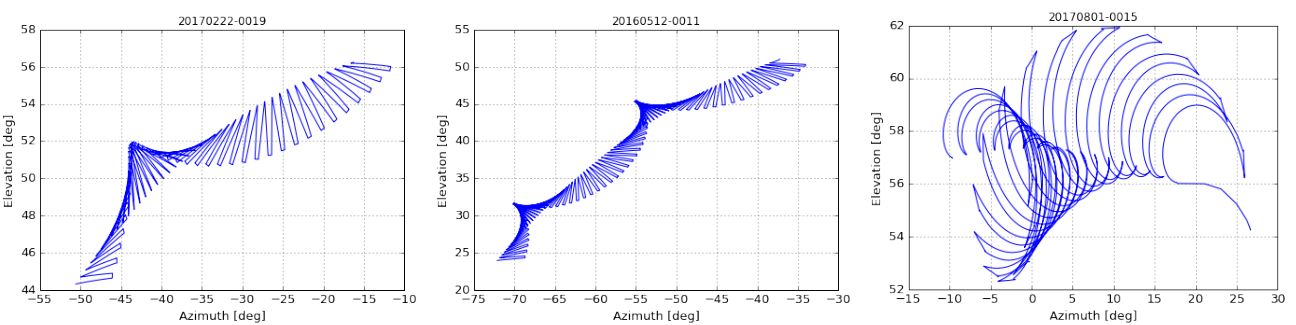
\includegraphics[width=6.2in]{c5/nn} %rasterscnn
	    %\vspace{5 mm}	   
	    \caption{The raster scanning patterns of three of the astro-holographic observations of MeerKAT. The title indicates the observation
ID. More information about the observations can be found in Table 1 and inside the text.}
	    \label{fig:rasterscn}
       \end{figure}
  \FloatBarrier 
% 

One major technique used in radio interferometry in order to measure the complex beam pattern of an antenna, is the holography. Generally, to produce a holography beam model, one radio telescope points constantly at a cosmic radio source whilst another telescope drifts across the source, usually in a raster scan form. We then obtain the complex beam pattern in terms of amplitude and phase by correlating the respective output powers with the reference antenna pointing at the same source. 

The main target source observed in this work is 3C 273 at a frequency of $1.365 \, \rm GHz$. In addition, Fig.~\ref{fig:rasterscn}  shows the patterns of the various raster scans used in this study. The 2017-02-22 observation was performed using three scanning antennas (M000, M012, M017) and one tracking antenna (M011). The scanning and tracking were performed from an elevation angle of $44^{\circ} \sim 57^{\circ}$, as seen in the figure, but we can also see that the beam is well-sampled within only a circular region of around $\sim 6^{\circ}$ diameter, centred at an elevation of $51.08^{\circ}$. The centre elevation is obtained from the average of the tracked elevations.
%
\noindent The holographic measurement of this radio interferometer is discussed extensively in  \citep{7305152}. Here, the observation is done not directly using the traditional raster scan approach as presented in \citep{1988A&A...190..353E} but instead, a complex scanning pattern like the one displayed in Fig.~\ref{fig:rasterscn}. This method is efficient because it cuts out the need for slew scans in the traditional way, and hence reduces the tracking period. However, the complex beams produced from this scheme are perturbed with undesirable radio frequency interference (RFI). The source of this disturbing noise can be resolving satellites and other physical radio emissions. Therefore, it is necessary to introduce a mathematical model to reconstruct these holography measured beams which is the main objective of this research, in order to denoise the data and achieve a high accuracy. In the original paper, we demonstrated three different numerical techniques namely; modified-Principal Component Analysis (PCA), Spherical Harmonics (SH) and Zernike Moment (ZM) to model the measured beams. For the purpose of this study, we focus on ZM only. Here, we want to further explore how the IM techniques discussed in Chapter~\ref{Chapter4} scale  to MeerKAT telescopes. Thus, instead of using {\tt OSKAR} to simulate perturbed fully polarized beams, we fit Zernike polynomials to MeerKAT holography measured beams using a particular number of Zernike coefficients with corresponding basis functions and then perturb the beams with the fit again, using different number of coefficients. We then simulate these reconstructed beams with the foregrounds to determine the leakage terms. 

The mathematical function of ZMs was originally developed to tactle wavefronts in optics. Now, the model has been adopted in many applications of image analysis such as image reconstruction~\citep{6243926}, image classification~\citep{1414392,khotanzad1990classification}, and image retrieval~\citep{7569541}. The orthogonal property of ZMs can depict an image with arbitrary number of polynomilas using the highest coefficients~\citep{teh1988image}. 

Next we present the mathematical model of ZM.
% Note, One of the MeerKAT beam models presented here is available through the openly accessible package EIDOS. 
%  the effects of the beam on HI intensity mapping 
 


\section{Methodology}	   \label{chap5:mkbeams}
%%

\subsection{Mathematical Basis of Zernike Polynomials}	   \label{chap5:zernike}
%%


Consider a wavefront  denoted by $\Phi_{w}(\rho,\theta)$, in polar coordinates $(\rho,\theta)$, to be a linear combination of Zernike polynomials over a circular unit, then this phenomenon can mathematically be expressed as:
\begin{equation}
 \Phi_{w}(\rho,\theta) = \sum\limits_{\rm \beta, \rm \alpha}^{M} C_{\rm \beta}^{\rm \alpha}Z_{\rm \beta}^{\rm \alpha}(\rho,\theta) %\sum\limits_{m = 0}^{n}
  \label{eq:wavefront}
\end{equation}
%

\noindent The \textit{basis of ZM} $Z_{\rm \beta}^{\rm \alpha}(\rho,\theta)$, in Equation~\ref{eq:wavefront} is defined as \citep{2015arXiv150607396F}: 
 
 \begin{equation}  \label{eq:zm}
Z_{\rm \beta}^{\rm \alpha}(\rho,\theta) = \left\{ \begin{array}{cc} 
                \Lambda_{\rm \beta}^{\rm \alpha} R_{\rm \beta}^{\lvert \rm \alpha \rvert}(\rho) \cos(\rho \rm \alpha \theta), & \hspace{3mm} \rm \alpha \geq 0 \\
                -\Lambda_{\rm \beta}^{\rm \alpha} R_{\rm \beta}^{\lvert \rm \alpha \rvert}(\rho) \sin(\rho \rm \alpha \theta), & \hspace{3mm} \rm \alpha < 0\\                
                \end{array} \right.
\end{equation}

\noindent The \textit{radial polynomial} $R_{\rm \beta}^{\lvert \rm \alpha \rvert}(\rho)$ and the \textit{normalisation factor} $\Lambda_{\rm \beta}^{\rm \alpha}$ in Equation~\ref{eq:zm} are respectively denoted as:\\

$R_{\rm \beta}^{\lvert \rm \alpha \rvert}(\rho)  = \sum\limits_{s = 0}^{\frac{\rm \beta - \lvert \rm \alpha \rvert}{2}}  \frac{(-1)^{s}(\rm \beta-s)! \rho^{\rm \beta-2s}}{s!\left[\frac{\rm \beta + \lvert \rm \alpha \rvert}{2} -s\right]!\left[\frac{\rm \beta - \lvert \rm \alpha \rvert}{2} -s\right]!}$, \quad 
$\Lambda_{\rm \beta}^{\rm \alpha} = \sqrt{\frac{2\rm \beta+1}{1+\delta_{\rm \alpha,\rm 0}}}$ \\
 
\noindent where $\delta_{\rm \alpha,\rm 0}$ is the Kronecker delta function such that $\delta_{0,0} = 1$ and $\delta_{\rm \alpha,\rm 0} = 0$ when $\rm \alpha \neq 0$.  The index $\rm \beta \geq 0$: $\rm \beta = 0, 1, 2, \ldots $ and 
for a specific $\rm \beta$, the index $\rm \alpha$ takes the values $\rm \alpha = -\rm \beta, -\rm \beta + 2, -\rm \beta + 4,  \ldots , \rm \beta$.
%%

\noindent The polynomials $Z_{\rm \beta}^{\rm \alpha}(\rho,\theta)$ are a set of complete orthogonal over a unit circle and this is conveniently represented in Equation~\ref{eq:zm} as the products of angular functions and radial polynomials. The orthogonality of this function makes the coefficients not to be dependent on one another \citep{charman2005wavefront,wyant1992basic} and hence, these coefficients are normally expressed in double $(\rm \beta, \rm \alpha)$ or single $(j)$ modes. The $\rm \beta$ mode characterises the order of aberration and mode $\rm \alpha$ represents the azimuthal frequency of the sinusoidal. The radius parameter, denoted $\rho$, is continuous over the range of $(0, 1)$ and this means the azimuthal component is continuous over the range of $\theta$, such that $ 0 \leq \theta \leq 2\pi $. Fig.~\ref{fig:rp} displays $8$ of such radial responses, where it can clearly be observed that the polynomials converge as they approach the edge of the unit disc. This also confirms that the Zernike polynomials of all orders are confined to the interval $(-1,1)$ as shown in Fig.~\ref{fig:d_indx}. 
%
% 

\begin{figure}
\begin{minipage}[H]{\linewidth}
      \centering
      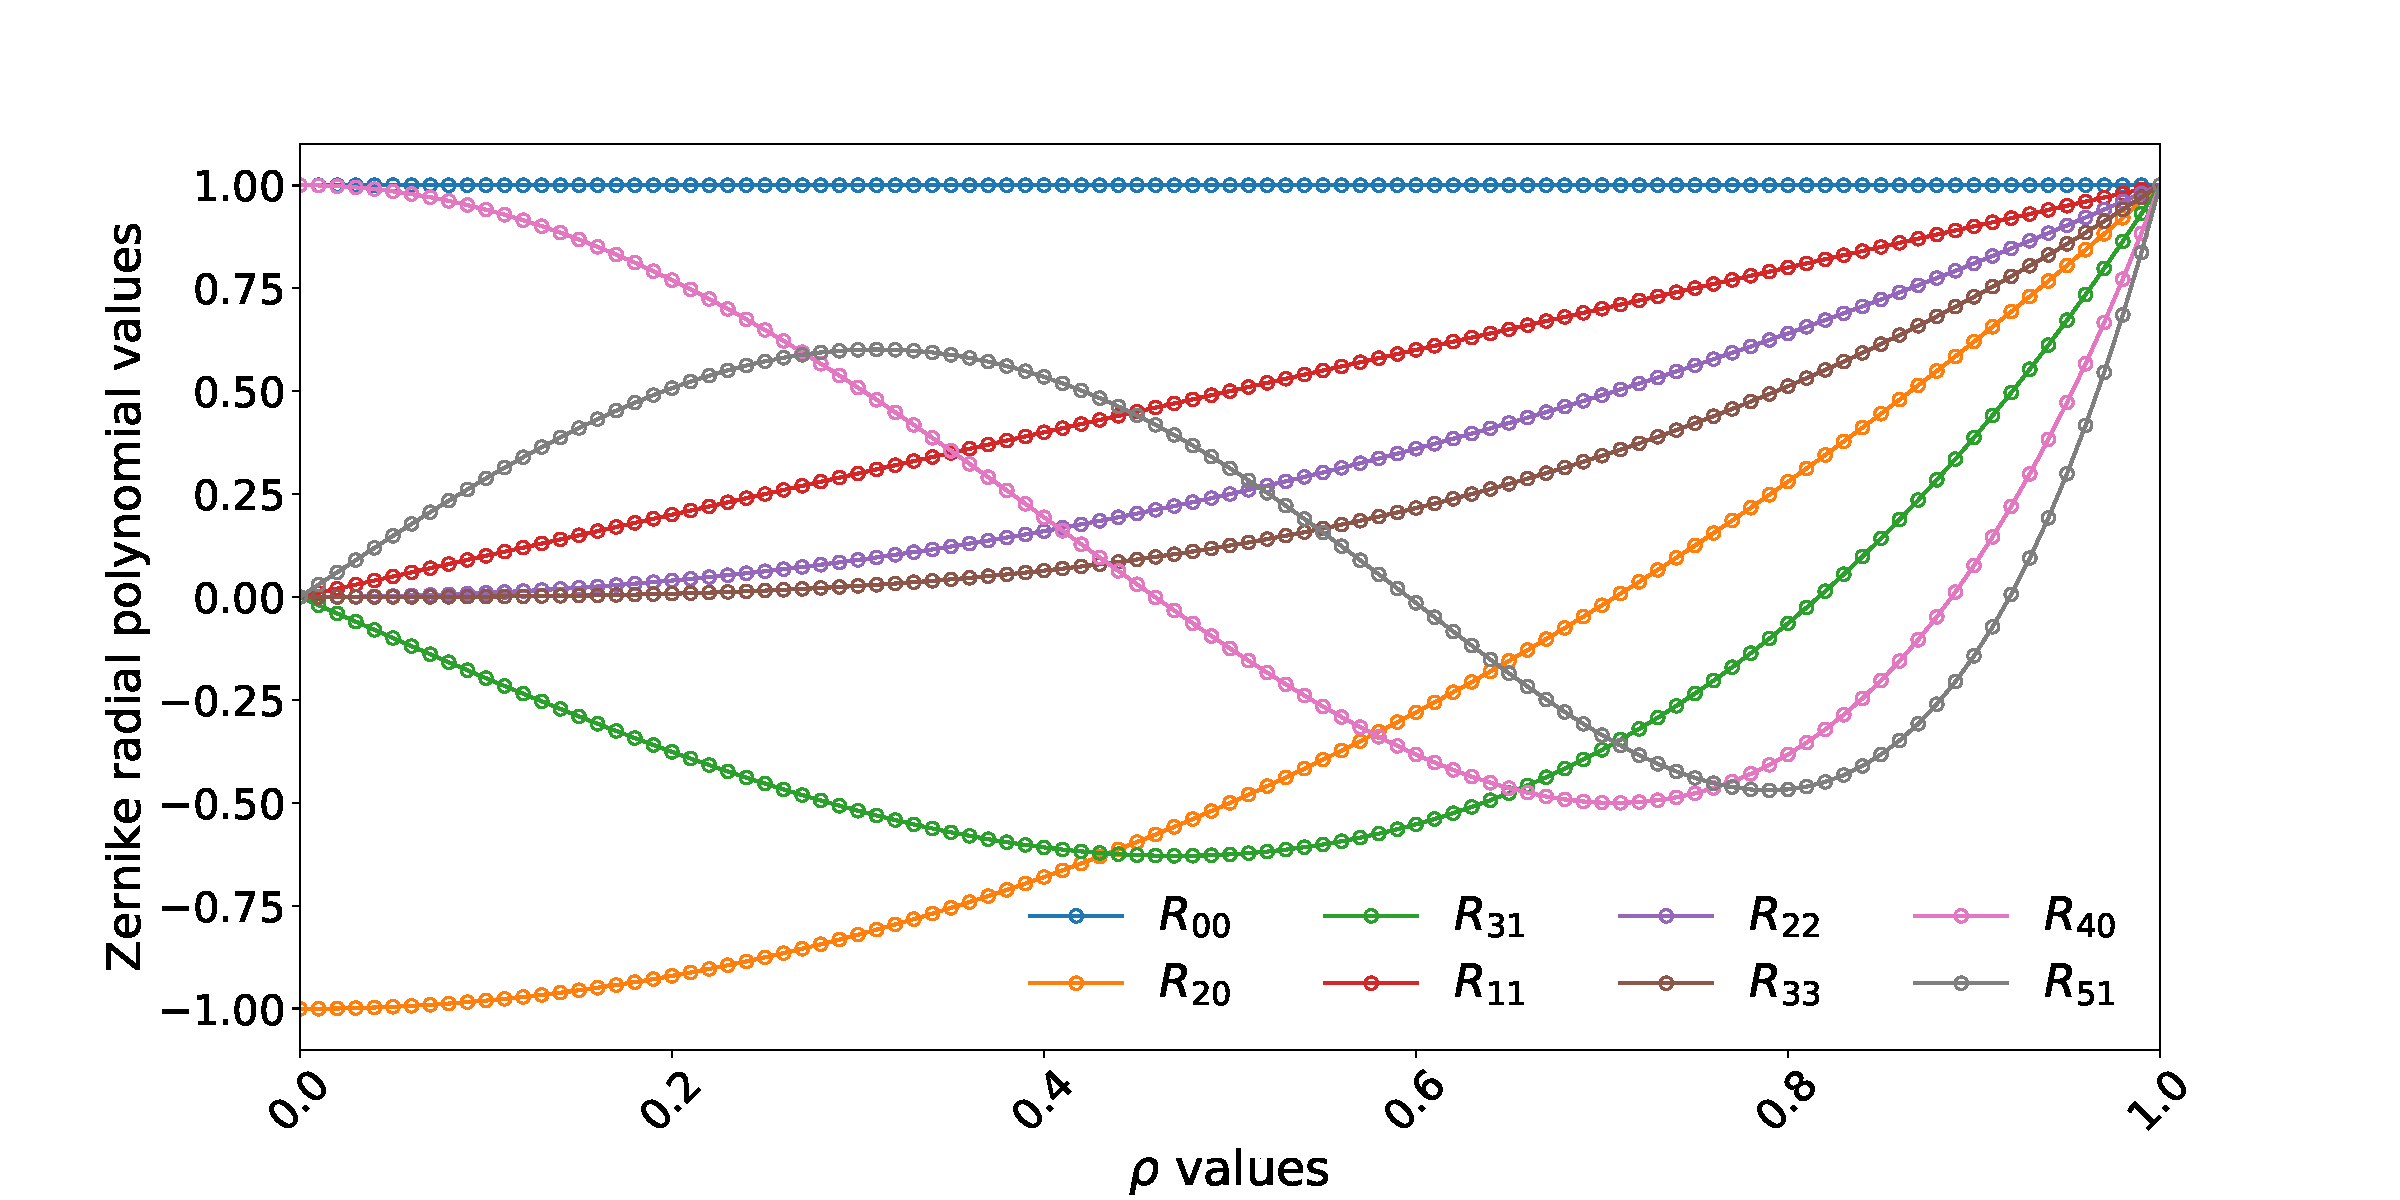
\includegraphics[width=\linewidth]{c5/rad_plot} %6.6in
      \end{minipage}
    \caption{\label{fig:rp} Expansion of eight orthogonal radial polynomial $R_{}^{\lvert \rm \alpha \rvert}(\rho)$ plots. Here, the value of unity can be obtained at the
outer edge, since $R_{\rm \beta}^{\lvert \rm \alpha \rvert}(1) = 1$.}
\end{figure}
\FloatBarrier
%%
%%

The surface plots in Fig.~\ref{fig:d_indx} depict the Zernike pyramid formed by the first $6$ levels. In the central column, the modes are invariant by rotation $(\text{i.e.} \, \rm \alpha=0)$ and hence, the column can be seen as a symmetry around the axis. On each level (i.e. same $\rm \beta$ value), the Zernike modes of opposite azimuthal frequency value have the same overall shape, but a different orientation. These pairs are required to enable any mode to be freely moved around $360^\circ$, by selectively adjusting the weight of each mode to obtain the desired orientation. Note, for further discussions on ZM, we can refer to these articles \citep{campbell2003new,lakshminarayanan2011zernike,1976JOSA...66..207N,wyant1992basic}.
% For further reading on ZM

%%

\begin{figure}
\begin{minipage}[H]{\linewidth}
\centering
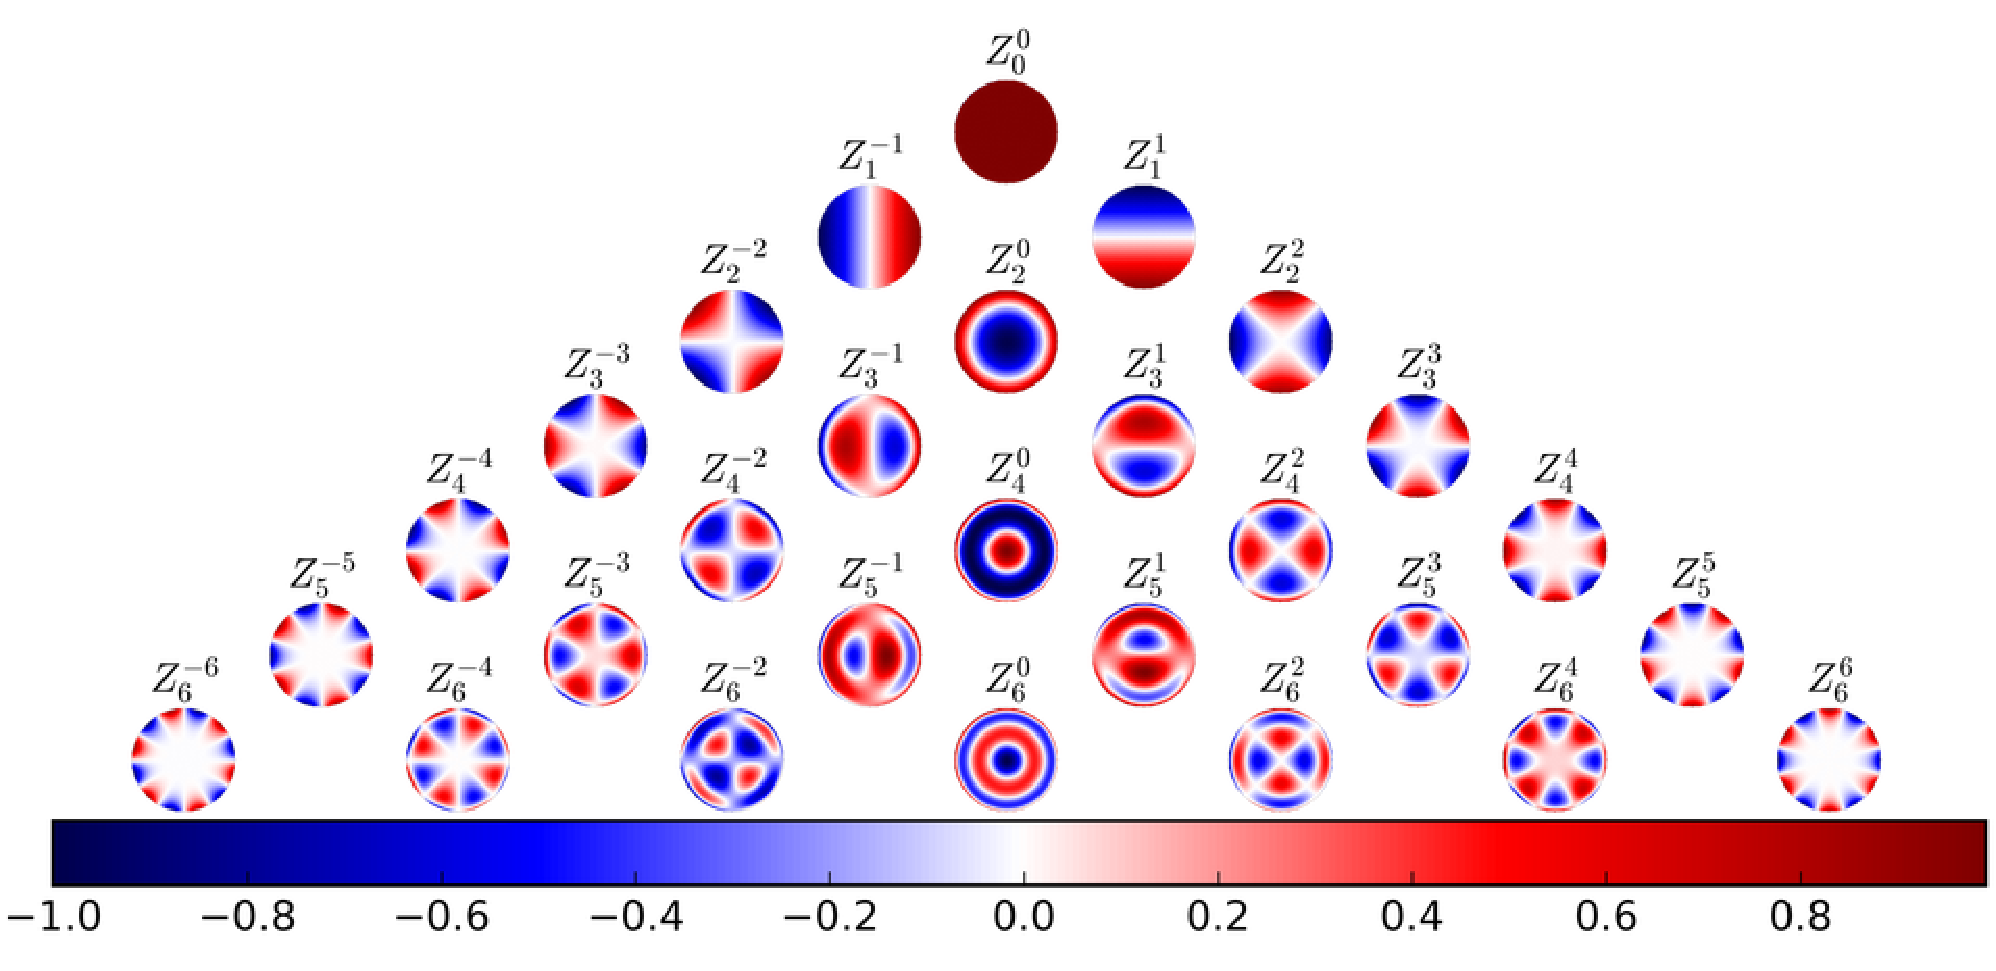
\includegraphics[width=\linewidth]{c5/kelazern}
\end{minipage}
\caption{\label{fig:d_indx} Representation of basis patterns of Zernike moments $Z_{\rm \beta}^{\rm \alpha}(\rho,\theta)$ of order $6$, plotted on a unit circle.}
\end{figure}
\FloatBarrier
%%

% %%
\subsection{Numerical Computation of Zernike Coefficients}	   \label{chap5:zcoff}
%%
In Equation~\ref{eq:wavefront}, the vector variable $C_{\rm \beta}^{\rm \alpha}$ (Zernike coefficient) is the only unknown factor that needs to be computed. 
Let $L$ denote the pixel positions of the measured beam $\Phi_{w}$, such that $\Phi_{w}^{\tau}(\rho_{\tau},\theta_{\tau})\mid_{\tau = 1,2,3,\ldots,L}$, where
$(\rho_{\tau},\theta_{\tau})$ is the corresponding pixel coordinate usually in polar form.  We then estimate the parameter $C_{\rm \beta}^{\rm \alpha}$ 
by rewriting Equation~\ref{eq:wavefront} in a simple form as expressed in Equation~\ref{eq:lsq} and then try to solve the least square problem using 
the matrix inversion approach. 
%%

\begin{equation}\label{eq:lsq}
 \bm{Z}_{\rm P \times L} \bm{C}_{\rm P \times 1} = \bm{\Phi}_{\rm L \times 1}
\end{equation}

\noindent where $\bm{\Phi}$ is the $L \times 1$ data array\footnote{{\tt The package numpy.ravel will return a neighbouring flattened array.}} that consists of  
the MeerKAT beams, $\bm{C}$ is the unknown coefficients of $ P \times 1$ array and  $\bm{Z}$ is the $P \times L$ matrix of polynomials that  provides 
the physical features of $\bm{\Phi}$. Expanding Equation~\ref{eq:lsq} we get;

\begin{equation}
{
 \begin{pmatrix}
   Z_{1}(\rho_{1},\theta_{1}) & Z_{2}(\rho_{1},\theta_{1}) & \cdots & Z_{P}(\rho_{1},\theta_{1})\\
   Z_{1}(\rho_{2},\theta_{2}) & Z_{2}(\rho_{2},\theta_{2}) & \cdots & Z_{P}(\rho_{2},\theta_{2})\\
    \vdots                    &     \vdots                 & \ddots &    \vdots  \\     
   Z_{1}(\rho_{L},\theta_{L}) & Z_{2}(\rho_{L},\theta_{L}) & \cdots & Z_{P}(\rho_{L},\theta_{L})
   \end{pmatrix}  \begin{pmatrix} c_{1}\\
				  c_{2}\\
				  \vdots\\
				  c_{L}
    
   \end{pmatrix} = 
   \begin{pmatrix}
    \Phi(\rho_{1},\theta_{1})\\
    \Phi(\rho_{2},\theta_{2})\\
    \vdots\\
    \Phi(\rho_{L},\theta_{L})\\
    
   \end{pmatrix}
  } \label{eq:lsq1}
  \end{equation}
%%
The resultant equation can be written in the form:

\begin{equation} \label{eq:invmthd}
 \bm{Z^{T}ZC} =  \bm{Z^{T}\Phi}
\end{equation}

\noindent such that, the desired Zernike coefficients can be obtained by direct inversion;

\begin{equation} \label{eq:invmthd2}
 \bm{C} =  \bm{(Z^{T}Z)^{-1}Z^{T}\Phi}
\end{equation}
%%

\noindent Therefore, given the basis patterns of Zernike polynomials and the corresponding coefficients, we can use these to reconstruct a particular wavefront.
In this study, the MeerKAT holography primary beams are used to represent the wavefront and then fit Zernike polynomials to reconstruct the measured beams.


%%%
% \subsection{Image Reconstruction} \label{chap5:img_reconstr}
%%
\subsection{Spatial Representation}	   \label{chap5:spatial}
%%

Note here that we represent the MeerKAT beams in the Jones matrix form as XX\footnote{{\tt Horizontal linearly unpolarized beam}}, XY\footnote{{\tt Horizontal linearly polarized beam}}, YX\footnote{{\tt Vertical linearly polarized beam }}, YY\footnote{{\tt Vertical linearly unpolarized beam}}. Therefore, these notations have the same meaning through out this chapter.

In this work, we select the strongest coefficient values to denoise the MeerKAT beams at $990\, \mathrm{MHz}$. The selection is done base on the modal number with a reduced value of root mean square deviation (RMSD: $[ 1/N \sum\limits_{k=1}^{N} \parallel \bm{D}_{\rm k}^{a} - \bm{D}_{\rm k}^{e}\parallel^{2}]^{1/2}$ where $N$ is the beam size, $\bm{D}_{\rm k}^{e}$ is the Zernike fitted beam and $\bm{D}_{\rm k}^{a}$ is the original beam) as reported in Fig.~\ref{fig:beams_mse}. The RMSD plots of XX and YY in Fig.~\ref{fig:beams_mse} (blue and red) show that, we can use $20$ strongest angular frequencies (m-modes) with $RSMD \approx 0.001$ to model the gain part of the original holography beams, since increasing the number of m-modes will not significantly improve the reconstructed model. The same explanation goes to the cross term plots (yellow and green), where we choose the $5$ strongest modes with $RSMD \approx 0.001$ and the respective coefficients to reconstruct.

The principal idea to adopt the Zernike scheme in this study is to decrease the number of feature parameters (i.e. Zernike basis functions)
required to depict the spatial morphology since generally, Zernike coefficients are highly sparse. If we use a smaller number of coefficients, there's the possibility that the modelled image  will not be well-fitted. In addition, if the number of coefficients is very high, there's the likelihood of over-fitting the modelled image. In this research, we cautiously choose the strongest number of coefficients by truncating the coefficients up to a given threshold parameter based on the RMSD value.
%%
%%
\begin{figure}
\begin{minipage}[H]{\linewidth}
\centering
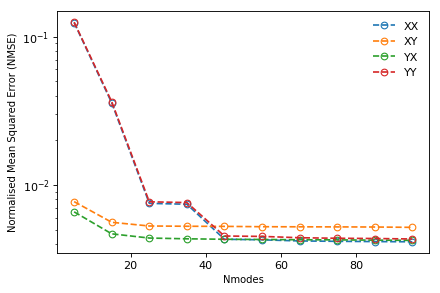
\includegraphics[width=\linewidth]{c5/mse_err3} %mkk/mse}
\caption{\label{fig:beams_mse} The expected value of the squared error loss  between the holography beam and the predicted beam model with respect to 
increase in the number of Zernike modes. (XX, YY) and  (XY,YX) are the linear polarization for the gain and cross terms of the Jones beams respectively.}
\end{minipage}
\end{figure}
\FloatBarrier
%%
We use this idea to reconstruct a 2D image from a Zernike fit. Here, all we need to have are the coefficients and the respective basis functions.
Fig.~\ref{fig:b20-5} shows a reconstructed MeerKAT beam model at a frequency of $990$ MHz for antenna M017. Note how the Zernike modelled beams (middle plots)
have de-noised the original beams. To test the goodness of fit of this model, we vary the number of Zernike coefficients and compare their residuals. The 1st $2$ plots in Fig.~\ref{fig:3rad} are the radial profile plots 
when we use the $5$ strongest coefficients for all the Jones terms and the $10$ strongest coefficients for all the Jones terms respectively. 
Note how the standard errors of these plots are higher than the 3rd plots which occur when we use the coefficients of $20$ and $5$  for the gain and cross terms respectively. This is confirmed when we also look at the distribution of the histogram plots in Fig.~\ref{fig:3hist}. Using $>5$ strongest coefficients to model the cross terms and  $<20$ strongest coefficients to model the gain terms will result in the perturbation of the beams. 

% 
%% Figs.~\ref{fig:3rad} and~\ref{fig:3hist}
% display the radial profile and a histogram of the distribution of different residual plots.
\begin{figure}
\begin{minipage}[H]{\linewidth}
\centering
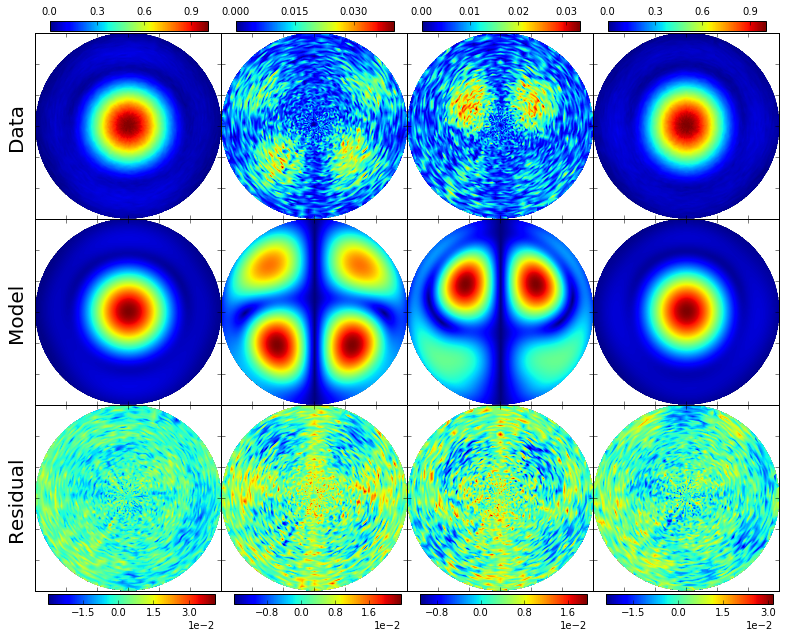
\includegraphics[width=\linewidth]{c5/2im/20-5}
\caption{\label{fig:b20-5} Zernike reconstructed MeerKAT beam model at $990\, \mathrm{MHz}$, using $20$ and $5$ strongest coefficients to model the gain and cross components respectively. The first and fourth columns are the amplitude beams of XX and YY respectively whilst the beams in the second and third columns are XY and YX correspondingly.}
\end{minipage}
\end{figure}
\FloatBarrier
%%


\begin{figure}[H] 
  \centering
     \begin{subfigure}[b]{\columnwidth} %{0.3\textwidth}%{\columnwidth}
%                 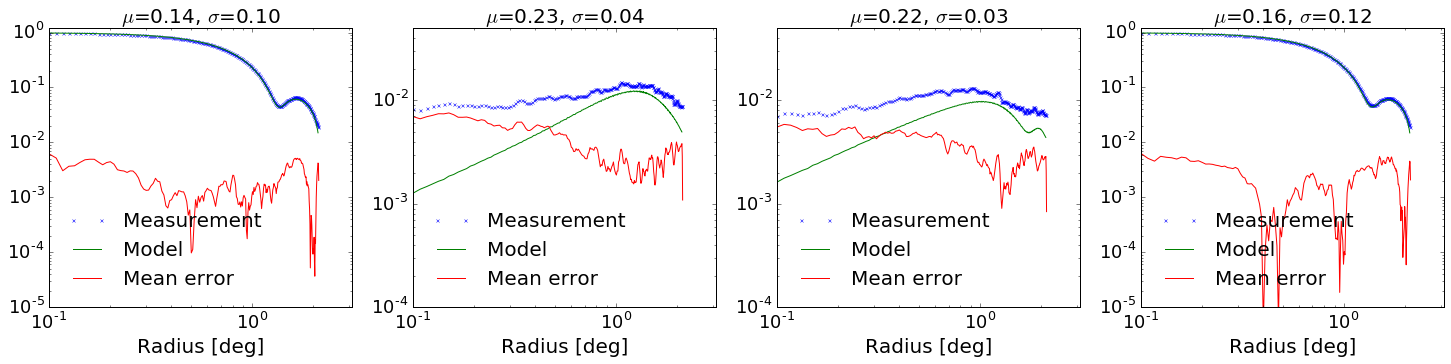
\includegraphics[width=\linewidth]{c5/2im/5-5r}
                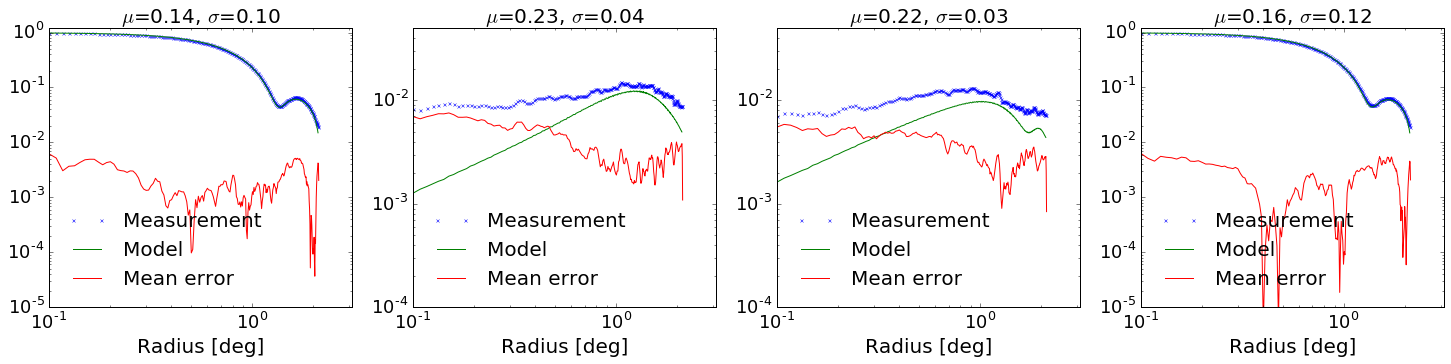
\includegraphics[height=1.6in]{c5/2im/5-5r}
                \caption{}
                \label{fig:A5a}
        \end{subfigure} \\ %\hfill
        %%
        \begin{subfigure}[b]{\columnwidth}%{0.3\textwidth} %{\columnwidth}
                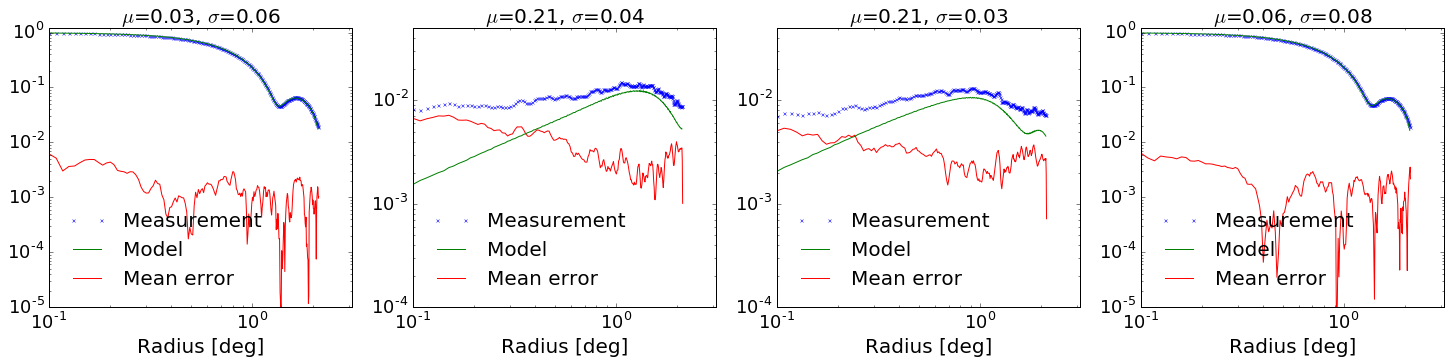
\includegraphics[height=1.6in]{c5/2im/10-10rd}
                \caption{}
               \label{fig:A5b}
        \end{subfigure}\\ % \hfill
        %%
        \begin{subfigure}[b]{\columnwidth}%{0.3\textwidth}%{\columnwidth}
                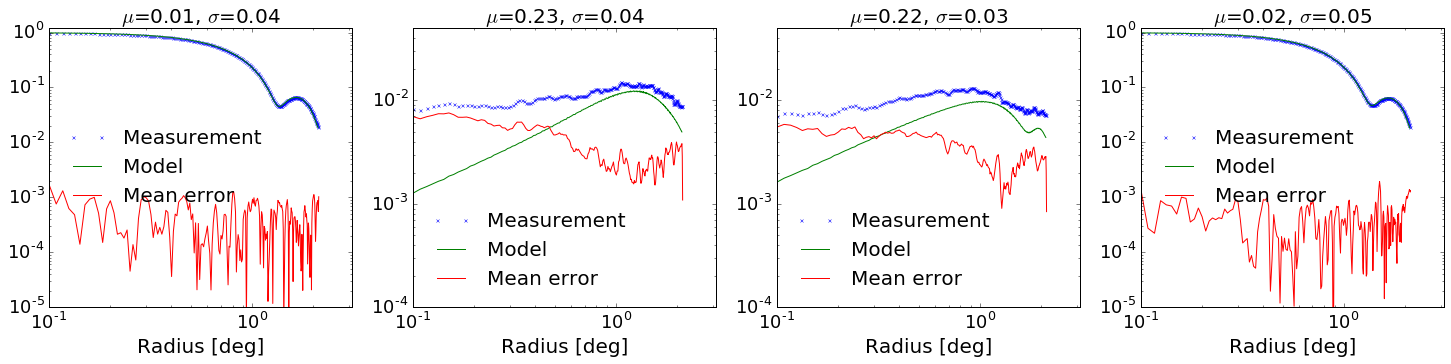
\includegraphics[height=1.6in]{c5/2im/20-5rd}
                \caption{}
               \label{fig:A5c}
        \end{subfigure}
        
        \caption{Radial profile of Fig.~\ref{fig:b20-5}. (a) Using $5$ strongest Zernike coefficients for the Jones components.  
        (b) Using $10$ strongest Zernike coefficients for the Jones components.
        (c) Using $20$ strongest Zernike coefficients for the gain components and $10$ strongest Zernike coefficients for the cross components.}
	     \label{fig:3rad}
  \end{figure}
  \FloatBarrier
 
\begin{figure}[H]
  \centering
     \begin{subfigure}{\columnwidth}
                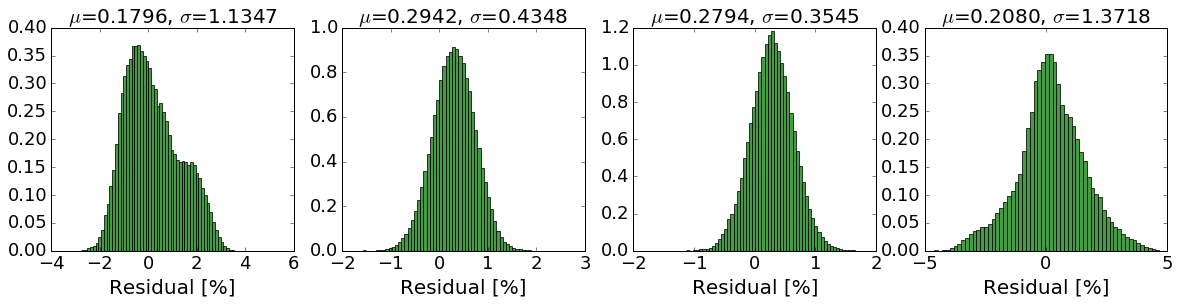
\includegraphics[width=\linewidth]{c5/2im/5-5h}
                \caption{}
                \label{fig:A10a}
        \end{subfigure} \hfill
        %%
        \begin{subfigure}{\columnwidth}
                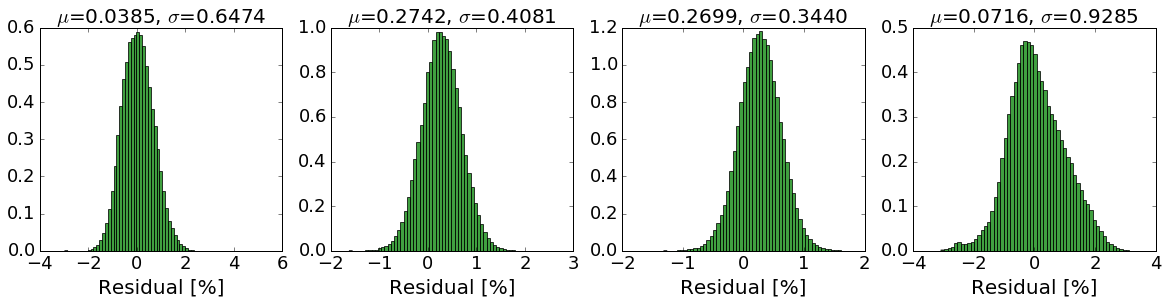
\includegraphics[width=\linewidth]{c5/2im/10-10h}
                \caption{}
               \label{fig:A10b}
        \end{subfigure} \hfill
        %%
        \begin{subfigure}{\columnwidth}
                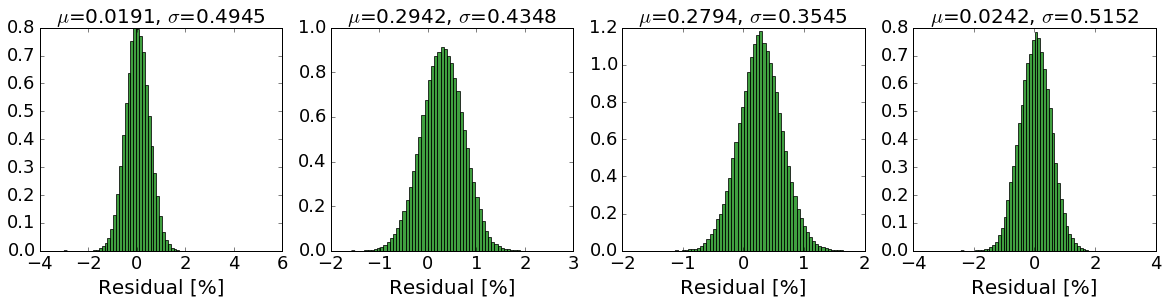
\includegraphics[width=\linewidth]{c5/2im/20-5h}
                \caption{}
               \label{fig:A10c}
        \end{subfigure}
        
        \caption{Histogram plots showing the residual distribution. (a) Plots obtained from using $10$ strongest Zernike coefficients for the Jones components.
        (b) Plots obtained from using $10$ strongest Zernike coefficients for the Jones components.
        (c) Plots obtained from using $20$ strongest Zernike coefficients for the gain components and $10$ strongest Zernike coefficients for the cross components.
	    }
	    \label{fig:3hist}
  \end{figure}
  \FloatBarrier

Next, we discuss how we reconstructed missing channels of the holography beams, using the DCT \enquote*{Discrete Cosine Transform} approach.
 %%
 
\subsection{Spectral Representation}	   \label{chap5:spectral}
%%

Most of the MeerKAT beams in the L-band are highly corrupted by RFI. The extremely damaged channels are within the following 
ranges;\\
$[(920, 960), (1125, 1305), (1463, 1492), (1520, 1630)]\, \rm MHz$.
We discard the measurements in these patches, and reconstruct the coefficients therein by interpolation from the surrounding unaffected
channels. The spectral interpolation and compression are done simultaneously using Discrete Cosine Transform (DCT) for the amplitudes
$A(\bm{\nu}) = |C(\bm{\nu})|$ of the complex coefficients, and a three-parameter sine wave for the sines and cosines of the corresponding phases
$\phi(\bm{\nu}) = \tan^{-1}[\rm Im(C)/\rm Re(C)]$.
We found the amplitude and phase to be the more natural parameters to model in case of linear polarization feeds, such as
that of MeerKAT, as opposed to circular polarization feeds, e.g. that of VLA, where modelling the real and imaginary
parts of the coefficients, in frequency, seemed to be more appropriate.
%%%%

In this work, we compute the amplitude of the coefficients by packing the damaged parts mentioned above with temporary values which is 
linearly interpolated from the uncorrupted nearby channels. We can easily do this by using the \enquote*{\tt numpy.interp} Python package.

The interpolated amplitudes $A(\bm{\nu})$ are then decomposed using DCT (of Type II) as
 
 \begin{equation}\label{eq:dctA}
 A_{\rm k} = \frac{2}{\sqrt{wN_{\rm \nu}}} \sum_{n=0}^{N_{\rm \nu}-1}  A_{\rm n}(\bm{\nu}) \cos\left[ \frac{\pi k (2n +1)}{2N_{\rm \nu}} \right]
\end{equation}
 
 \noindent for $0 \leq  k < N_{\rm \nu}$ where $w = 4$ when $k = 0$ and $w = 2$ otherwise. Subsequently, we select the strongest $N^d$ DCT coefficients 
 and put the rest to zero resulting in the sorted coefficients $A'$ which, in turn, are used to reconstruct a smooth
spectral model of the amplitudes by Inverse DCT (same as DCT of Type III) as
\begin{equation}\label{eq:dctB}
 \hat{A}_{\rm n}(\bm{\nu}) = \frac{A'_{\rm 0}}{N_{\rm \nu}} + \sqrt{\frac{2}{N_{\rm \nu}}}+ \sum_{n=0}^{N_{\rm \nu}-1}  A'_{\rm k} \cos\left[ \frac{\pi n}{N_{\rm \nu}}(n+1/2) \right]
 \end{equation}
 for $0 \leq n < N_{\rm \nu}$.
 
The spectral profile in Fig.~\ref{fig:se_ampl} displays the amplitude of the Zernike coefficients where the dense dotted points are the fitted beams with missing channels whilst
the thin dotted lines are the interpolated beams obtained from $\hat{A}_{\rm n}(\bm{\nu})$ in Equation~\ref{eq:dctB}. The bad channels (missing gaps) in the plots are represented 
as light-gray vertical dashes. Here, we show in the descending order the strongest coefficients and the corresponding activated basis patterns that are unique in the reconstruction 
of all the channels (from $[856,1700]$ MHz). The plots in Fig.~\ref{fig:implota} represent the amplitude component of the horizontal linearly unpolarized beam (XX) of the Jones 
elements (usually referred to as the gain term) whilst Fig.~\ref{fig:implotb} represent the cross term (XY) of the Jones elements. The thick-gray dashes in Fig.~\ref{fig:implota}
are fiducial markings used to distinguish the activated basis functions whose coefficients are above $\sim 10 \%$. In our case, these are 
$Z_{\rm 2}^{0}, Z_{\rm 4}^{0}$ and  $Z_{\rm 6}^{0}$, and can be located at the principal axis of Fig.~\ref{fig:d_indx}. Their official names 
in \cite{lakshminarayanan2011zernike} are defocus ($Z_{\rm 2}^{0}$), $\rm 1^{st}$ spherical ($Z_{\rm 4}^{0}$) and $\rm 2^{nd}$ spherical ($Z_{\rm 6}^{0}$). Note that these 
basis functions are activated because we can observe from the plots that the ripple effect in the MeerKAT beams (XX) looks more stable across all frequencies, but this is 
not always the case for all antennas as we shall witness this change effect in SKA1-mid beams in the next chapter. On the other hand, the strongest basis patterns used in 
Fig.~\ref{fig:implotb} are $Z_{\rm 4}^{-2}, Z_{\rm 7}^{-1}, Z_{\rm 6}^{-2}, Z_{\rm 2}^{-2}, Z_{\rm 8}^{-2}$ and $Z_{\rm 5}^{-1}$ which are mostly 
composed of Zernike functions such as astigmatism ($Z_{\rm 4}^{-2}, Z_{\rm 6}^{-2}, Z_{\rm 2}^{-2}, Z_{\rm 8}^{-2}$) and coma ($Z_{\rm 7}^{-1}, Z_{\rm 5}^{-1}$). These patterns
are well defined for the representation of the solid cloverleaf patterns in the cross terms (XY) of MeerKAT beams. Note that the basis patterns in Fig.~\ref{fig:se_ampl} are the
same for the other components in the Jones matrix, thus, the component YY can be modelled with other patterns in Fig.~\ref{fig:implota} and YX uses the Zernike functions in 
Fig.~\ref{fig:implotb}. The MSE plots in Fig.~\ref{fig:beams_mse} confirm this too.
%%

 \begin{figure}
\begin{minipage}[H]{\linewidth}
\centering
    \begin{subfigure}[b]{1.0\textwidth}
	      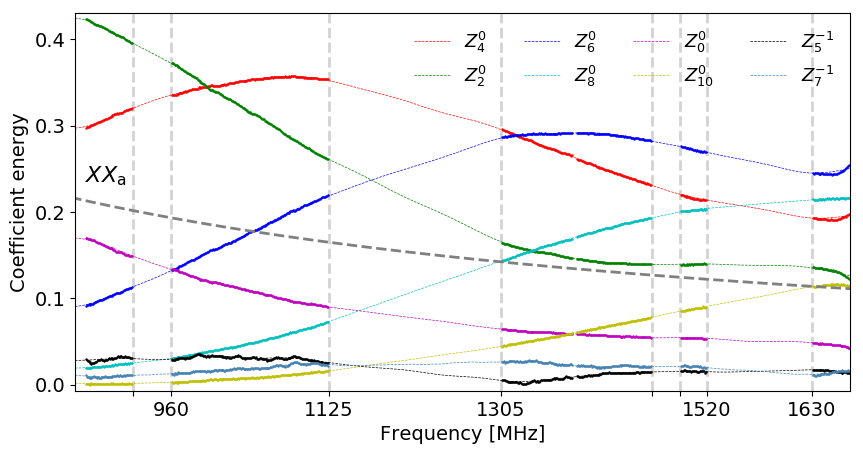
\includegraphics[width=\textwidth]{c5/m_xxa}               
	      \caption{}                
	      \label{fig:implota}
      \end{subfigure}       
      \begin{subfigure}[b]{1.0\textwidth}
	      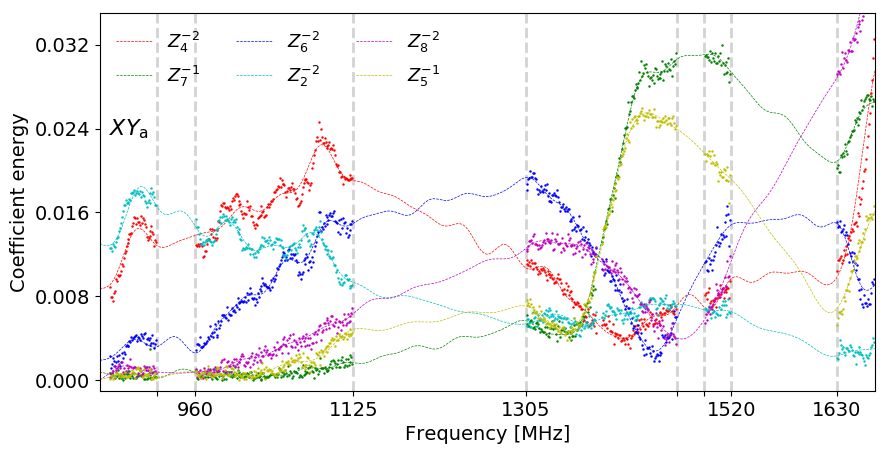
\includegraphics[width=\textwidth]{c5/m_xya}                
	      \caption{}               
	      \label{fig:implotb}
      \end{subfigure}        
	\end{minipage}
      \caption{\label{fig:se_ampl} Spectral representation of the amplitude of MeerKAT primary beams for L band. The light-gray vertical dashes are the missing gaps due to high RFI whilst the thin dotted lines are the DCT plots used to correct the bad channels for the respective Jones terms [XX (top) and XY (down)].}
	\end{figure}
\FloatBarrier
%
% \begin{figure}[H]{\columnwidth}
% \centering
% 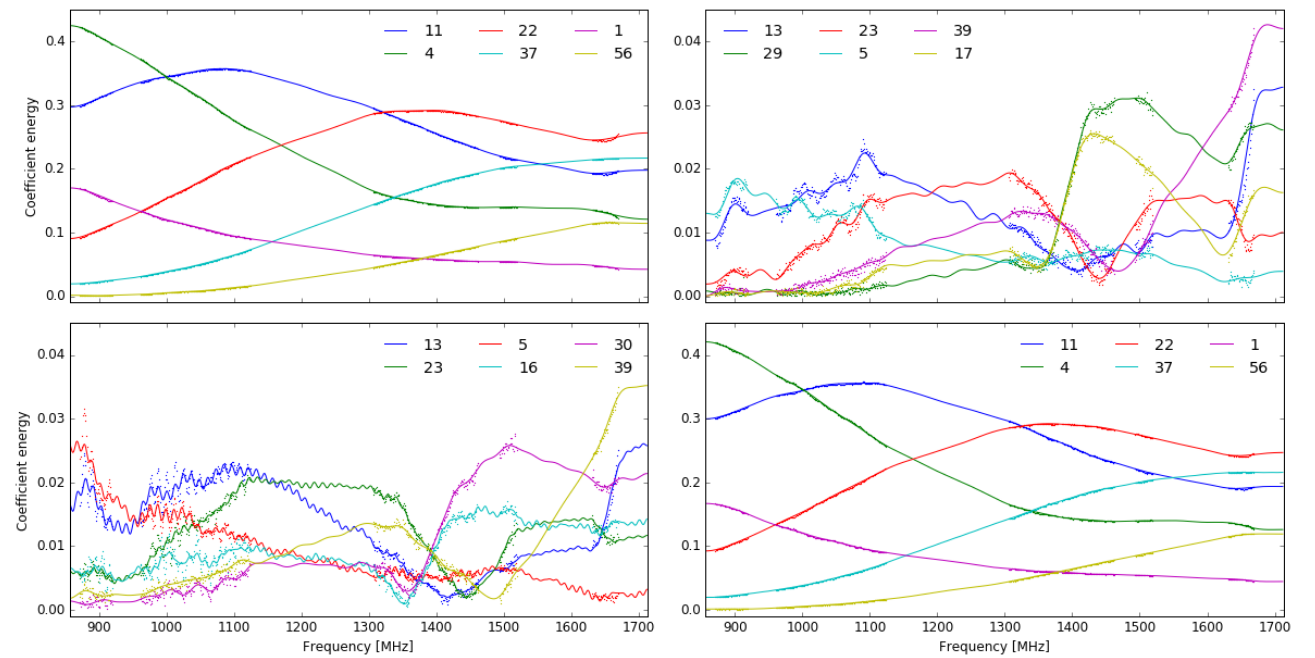
\includegraphics[height=3in]{/c5/spectral-mod/ampl}
% \caption{\label{fig:se_ampl} Spectral representation of the amplitude of MeerKAT primary beams for L band.
%                                      The dotted lines are the Zernike plots with missing frequency channels due to high RFI whilst
%                                      the solid lines are the DCT plots used to correct the bad channels 
%                                      for the respective Jones terms [XX (upper-left), XY (upper-right), YX (lower-left), YY (lower-right) ].}
% \end{figure}
% \FloatBarrier
%%


%%
\begin{figure}
\begin{minipage}[H]{\linewidth}
\centering
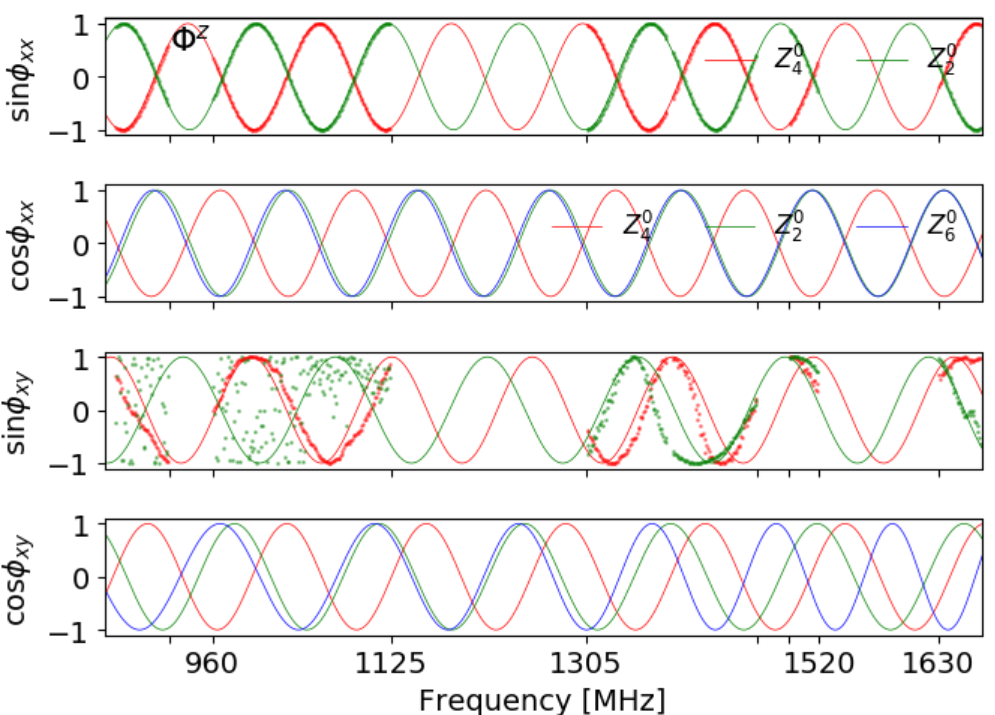
\includegraphics[width=\linewidth]{/c5/phase_angle}
\caption{\label{fig:sp_phse} Spectral representation of the phase of MeerKAT primary beams for L band.
                                     The thick dotted lines are the Zernike plots with missing frequency channels due to high RFI whilst
                                     the solid lines are the Sine and Cosine plots used to correct the bad channels 
                                     for the phase terms of XX and XY.}
      \end{minipage}
\end{figure}
\FloatBarrier
%%

\noindent In addition, we apply the sine wave with parameters $\alpha, \beta$ and $\gamma$ to model the beam phase:
 \begin{equation}\label{eq:phs}
  \zeta(\upsilon) = \sin(2\pi \frac{\nu}{\alpha} + \beta \cos 2\pi \frac{\nu}{\gamma}) 
 \end{equation}

 \noindent Therefore, using the \enquote*{\tt lmfit.minimize} Python package with the Nelder-Mead method,  we can then 
 fit $\zeta(\upsilon)$ to $\sin \phi(\nu)$ and $\cos \phi(\nu)$ to obtain the plots in Fig.~\ref{fig:sp_phse}. Here, the missing channels are reconstructed by taking  the Sine and Cosine of the imaginary and real parts of the Jones terms accordingly. Note how the Sine and Cosine functions actually predicted the Zernike coefficients for the  phase beams of XX. Nevertheless, we obtained some deviations for the imaginary part of the cross term (XY) even though the real part actually predicted the missing gaps correctly.  

We now discuss the results obtained when we simulate the foregrounds with the above modelled beams to compute  the polarization leakage when performing an IM experiment.
% 

%% 
\section{Results and Discussion}	   \label{chap5:RnD}
%%

 The convolved maps presented in Fig.~\ref{fig:mz} are a repetition of the simulation we discussed in Section~\ref{sec:convolution}.  Here the reconstructed MeerKAT primary beams are transformed from the Jones terms into complete Mueller beams. These Mueller beams are then used to convolve the foregrounds maps  in Fig.~\ref{fig:f990}. The 1st row is the true measured maps when the modelled beams used are constructed with $20$ and $10$ strongest coefficients for the  gain and cross terms respectively. The next $2$ rows are the perturbed measured maps  when we fully model the beams with $5$ and $10$ Zernike coefficients in a respective manner. The remaining rows are the residual maps between the true and the perturbed  measured maps. Note carefully how these scaled measured maps (both true and perturbed) are very similar but the actual differences are shown in the error maps.
 %%
 
 \begin{figure}
 \begin{minipage}[H]{\linewidth}
      \centering      
      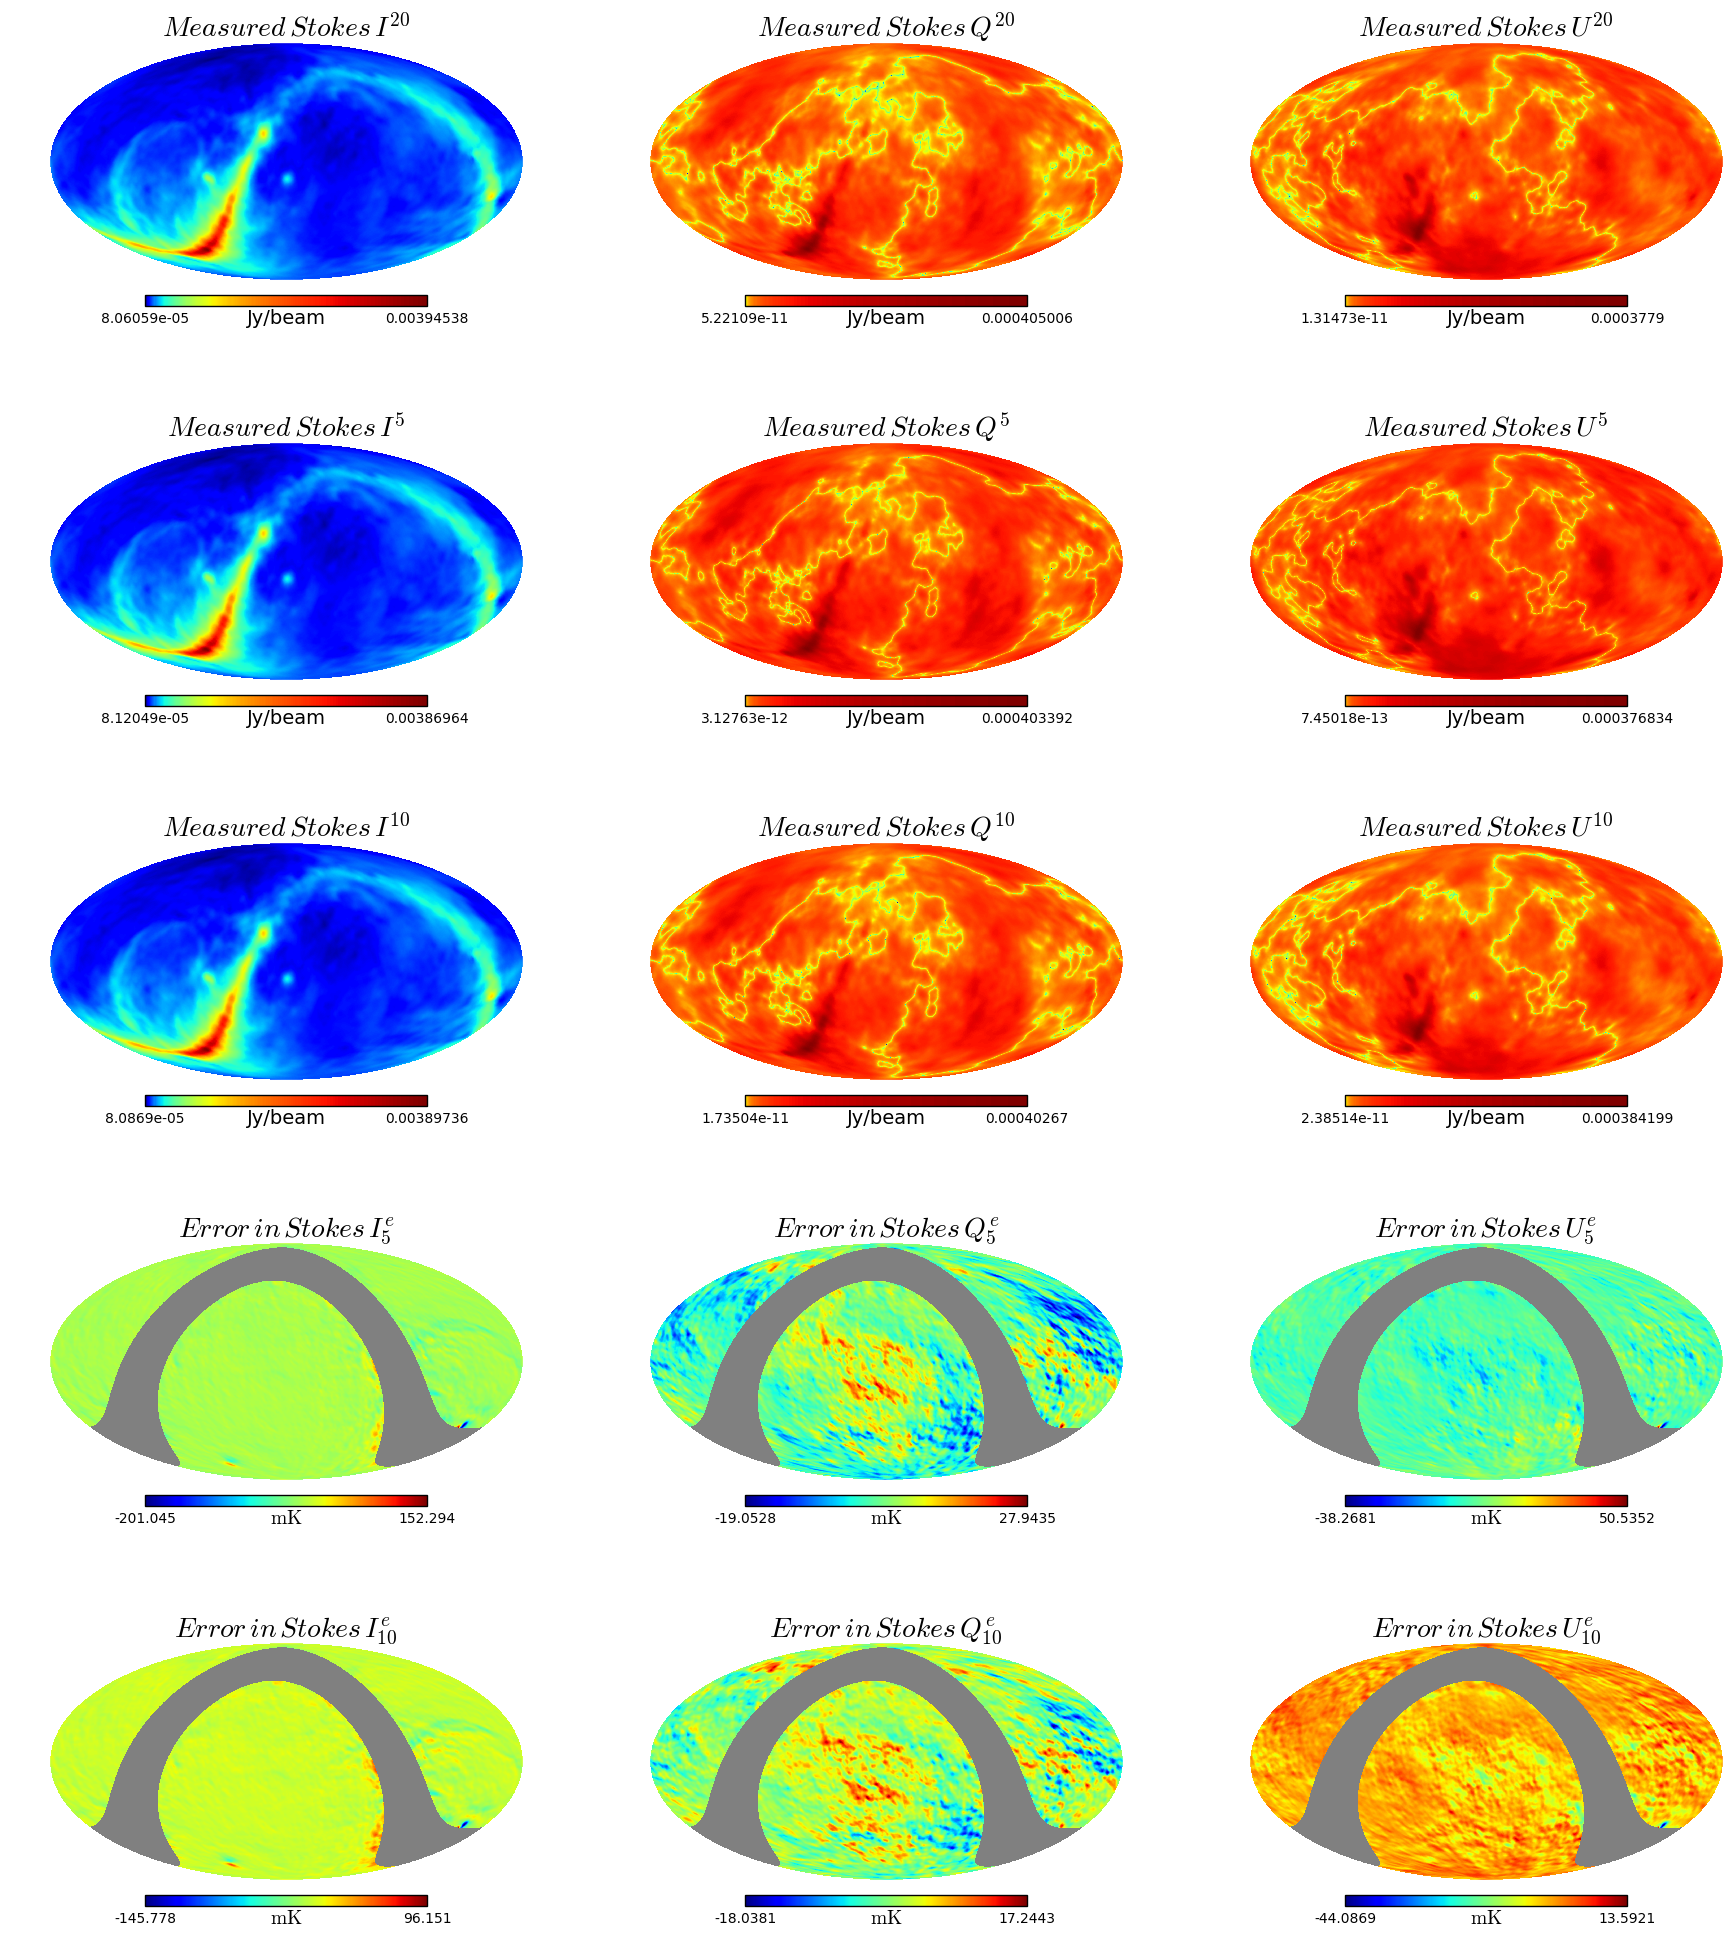
\includegraphics[width=\linewidth]{/c5/mkk/m/mk_fconv}     
     \caption{ \label{fig:mz}  Measured Stokes $I, Q$ and $U$ convolved with reconstructed MeerKAT beam models with corresponding error maps. $1^{\rm st}$ row: These are maps convolved with Zernike beams with $20$ highest coefficients.
     $2^{\rm nd}$ row: These are maps convolved with Zernike beams with $5$ highest coefficients.
     $3^{\rm rd}$ row: These are maps convolved with Zernike beams with $10$ highest coefficients. The $4^{\rm th}$ and  $5^{\rm th}$ rows are the corresponding residual maps between the $1^{\rm st}$ and  $2^{\rm nd}$ rows and between the $1^{\rm st}$ and  $3^{\rm rd}$ rows.} 	   
	 \end{minipage}
    \end{figure}
%%


 The spectra plots displayed in Fig.~\ref{fig:hI} show how the HI signal power is estimated when we correct the errors in the reconstructed beams and vice versa. If the errors in the reconstructed beams are corrected in Stokes $I$ 
as shown in the left plot, then the HI signal power is estimated at a multipole moment of $l \backsimeq 25$ and if the error is not corrected at all 
in Stokes $I$ but the intrinsic polarization leakage ($|Q + iU|_z$) in $I$ is known, then the HI signal power is estimated at a multipole moment of $l \backsimeq 100$. This multipole moment is about $4$ orders of magnitude greater than the foreground at lower scales. However, if the intrinsic  $|Q + iU|_{z} \longrightarrow I$ is corrected, then the HI signal power is evaluated at a multipole moment of $l \backsimeq 50$. This multipole moment is about $2$ orders of magnitude greater than the foreground at lower scales.
 % %%

\begin{figure}
 \begin{minipage}[H]{\linewidth}
      \centering      
      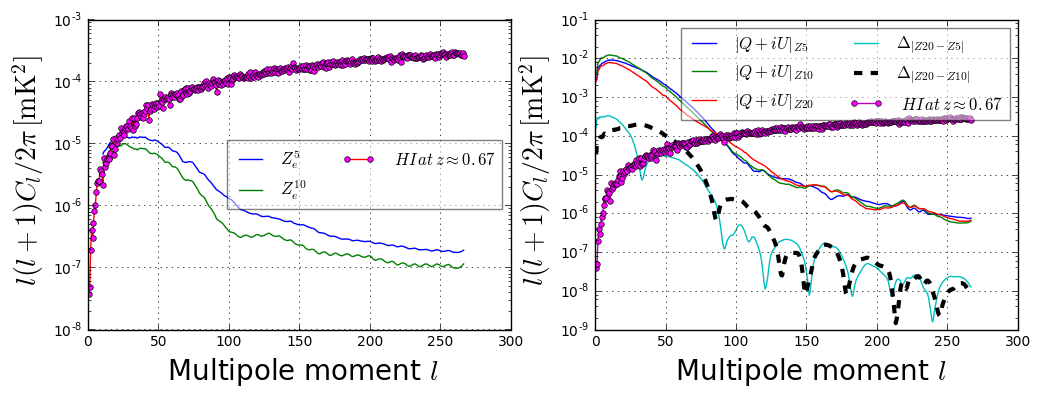
\includegraphics[width=\linewidth]{/c5/mkk/m/mk_hi_sim1}     
     \caption{ \label{fig:hI}    The distribution of angular power plots displaying the errors due to perturbed Zernike fits in Stokes $I$ map (left plots) and 
     the intrinsic leakage in $I$ (right plots) affect the $21$ cm signal (solid circular spectrum plot).}
     \end{minipage}	    
    \end{figure}
%%

\section{Conclusion}	   \label{chap5:concs}
%%
% 

In this chapter, we have clearly shown that the Zernike decomposition is a very well-fitted model for IM experiments. The model was able to reconstruct
the MeerKAT L-band holography measured beams. The reconstruction of the true modelled beam was done by using the strongest Zernike coefficients and the corresponding
basis functions. In order to distort the true modelled beams, the study used more and less strong Zernike coefficients with the respective basis functions
to perturb the modelled beams. In addition, to measure the HI signal power spectrum, the study performed an IM experiment by convolving these modelled beams 
with the foregrounds of the sky. The following are the key outcomes in this research:

\begin{itemize}
\item The true modelled beams were reconstructed with $20$ strongest Zernike coefficients for the gain terms of the Jones matrix (XX and YY) and 
$5$ strongest coefficients for the cross terms of the Jones matrix (XY and YX). The maximum standard error obtained from the reconstruction is $\backsimeq 0.05$.

\item The corrupted modelled beams were generated with $5$ strongest coefficients for all the Jones matrix terms (XX, XY, YX and YY). The second distortion was done
with $10$ strongest coefficients for all the Jones matrix terms (XX, XY, YX and YY). The maximum  standard errors obtained are $0.12$ (for using $10$ strongest coefficients)
and  $0.08$ (for using $10$ strongest coefficients).

\item The astigmatism and coma Zernike functions turn out to have the strongest coefficients to model the cloverleaf nature for the cross terms (XY, YX) of MeerKAT beams whilst 
the piston and spherical basis functions prove to be the best model for the gain terms (XX, YY). 

% \item Currently, there

\item The HI signal power is measured at a multipole moment of $l \backsimeq 25$ if we correct the beam errors in Stokes $I$ and at a multipole moment of $l \backsimeq 100$ if we do not correct the beam errors in $I$. 
\end{itemize}

\noindent  In summary,  the primary beam is critical in IM experiments and therefore, the plots in Fig.~\ref{fig:beams_mse} have shown that we can decompose the beams with an arbitrary number of Zernike polynomials but then we must select the highest coefficients up to a given threshold parameter based on the RMSD value. Hence, with a good Zernike model of the primary beams, we can actually measure the amount of foregrounds that have leaked from intensity into polarization.

